\appendixsection{Диаграмма контейнерного развёртывания}

В приложении приведена схема контейнерного развёртывания проекта.
Рисунок~\ref{fig:a1} использует подготовленный в каталоге \texttt{report}
архитектурный артефакт и показывает состав runtime-окружения: backend,
PostgreSQL, административную панель, прокси-слой и внешний Bitcoin RPC узел.

\begin{figure}
    \centering
    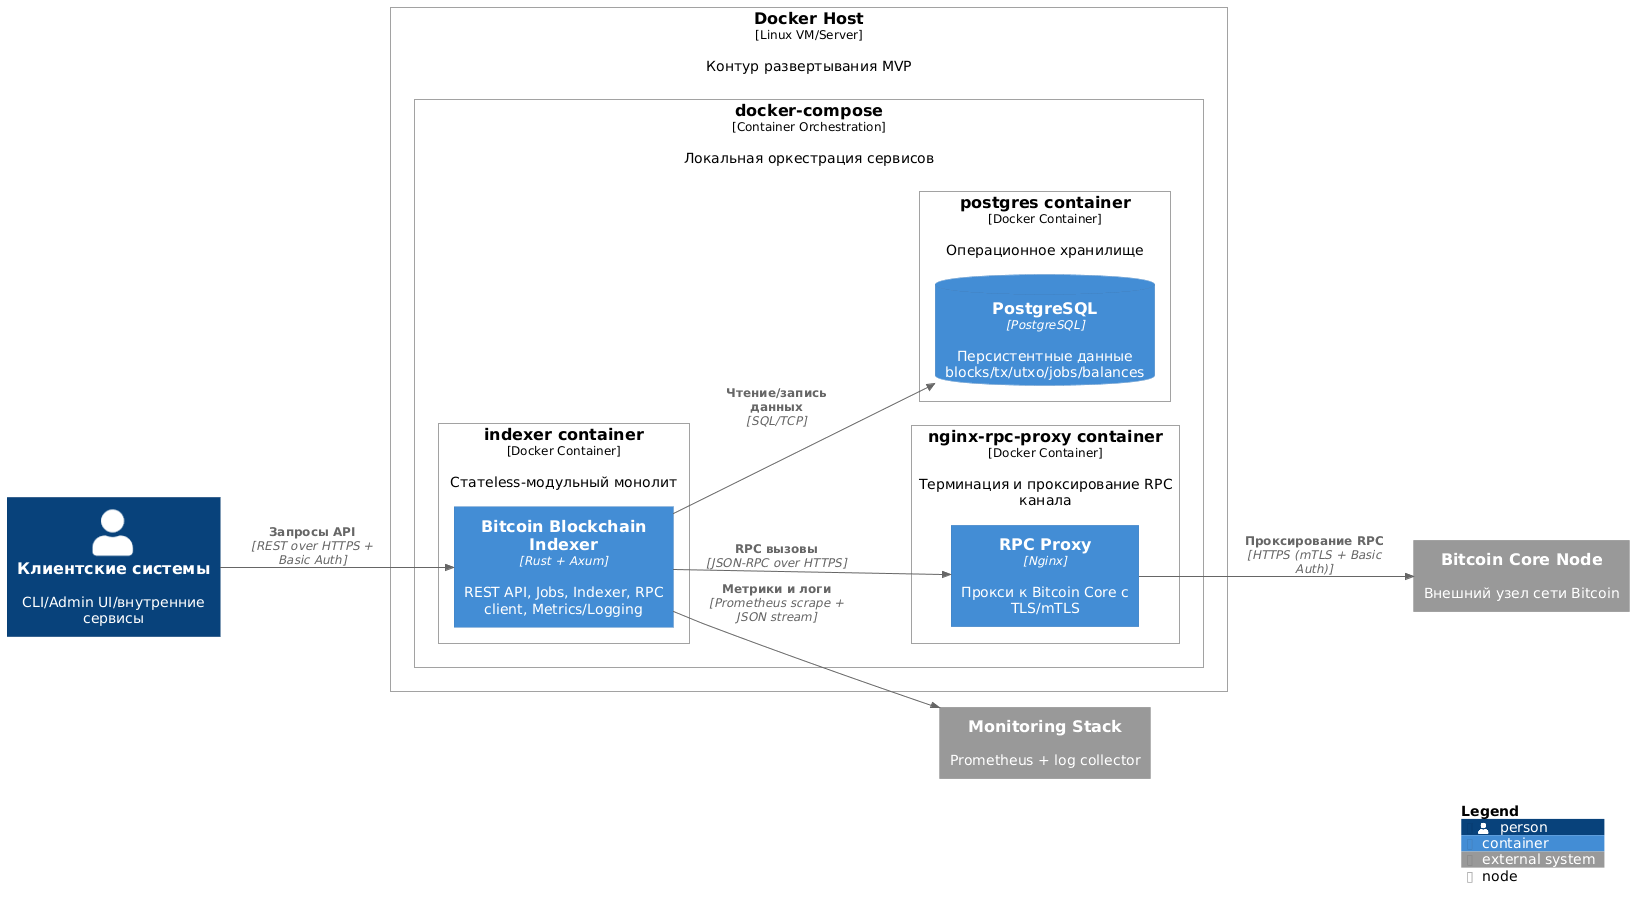
\includegraphics[width=\linewidth]{../report/c4/C4_Deployment_Architecture.png}
    \caption{Контейнерное развёртывание системы}
    \label{fig:a1}
\end{figure}
